\documentclass{article}
\usepackage{geometry}
\geometry{
	a4paper,
	left=2.5cm,
	right=2.5cm,
	top=2.5cm,
	bottom=2.5cm,
	headheight=13.6pt
}
% 最简单、最稳定的中文方案（自动适配系统，永不报错）
\usepackage[UTF8, scheme=plain]{ctex}
% 设置英文默认字体为 Times New Roman
\usepackage{fontspec}
\setmainfont{Times New Roman}
\usepackage{amsmath}
\usepackage{amssymb}
\usepackage{booktabs}
\usepackage{caption}
\usepackage{setspace}
\doublespacing
\setlength{\parskip}{4pt}
\usepackage{array}
\usepackage{listings}
\usepackage{graphicx}
\usepackage{enumitem}
\usepackage{subcaption}
\usepackage{multirow}
\usepackage{mathrsfs}
\usepackage{bm}
\usepackage{xcolor}
\usepackage{colortbl}
\usepackage{tikz}
\usepackage{tikz-3dplot}
\usetikzlibrary{
	arrows.meta,
	calc,
	patterns,
	decorations.pathmorphing,
	backgrounds,
	positioning,
	fit,
	shapes.geometric,
	intersections,
	through,
	angles,
	quotes,
	plotmarks
}
%目录超链接
\usepackage{hyperref}
\hypersetup{
	colorlinks=true,
	linkcolor=black,
	filecolor=magenta,
	urlcolor=cyan,
}
\usepackage{tocloft}
\setlength{\cftbeforesecskip}{2ex}
\setlength{\cftbeforesubsecskip}{1ex}
\setlength{\cftbeforesubsubsecskip}{1ex}
% 定义代码颜色
\definecolor{codegreen}{rgb}{0,0.6,0}
\definecolor{NavyBlue}{RGB}{0,0,128}
\definecolor{PineGreen}{RGB}{1,121,111}
% 配置 listings 环境
\lstset{
	language=TeX,
	tabsize=4,
	captionpos=b,
	numbers=left,
	numbersep=1em,
	sensitive=true,
	showtabs=false,
	frame=shadowbox,
	breaklines=true,
	keepspaces=true,
	showspaces=false,
	showstringspaces=false,
	breakatwhitespace=false,
	basicstyle=\ttfamily\normalsize,
	keywordstyle=\color{NavyBlue},
	commentstyle=\color{codegreen},
	numberstyle=\color{black},
	stringstyle=\color{PineGreen!90!black},
	rulesepcolor=\color{red!20!green!20!blue!20},
	escapeinside={/@}{@/},
}
% 自定义颜色
\definecolor{LightGreen}{rgb}{0.9, 0.95, 0.9}
\definecolor{LightBlue}{RGB}{229, 238, 255}
\definecolor{LightPink}{RGB}{255, 229, 237}
\definecolor{DarkRed}{RGB}{169,0,0}
\definecolor{DarkGreen}{RGB}{0,110,12}
\definecolor{SkyBlue}{RGB}{0,114,255}
% 自定义环境 无缩进
\newenvironment{knowledge}[1]{%
	\noindent{%
		\normalfont\bfseries\color{DarkRed} #1}\hskip 0.5em%
	\color{DarkRed}%
}{%
	\par\color{black}%
}
\newenvironment{question}[1][]{%
	\noindent
	\ifx\relax#1\relax\else
	{%
		\normalfont\color{DarkGreen} #1}\hskip 0.5em%
	\fi
	\color{DarkGreen}%
}{%
	\ifhmode\fi\color{black}%
}
\newcommand{\category}[1]{%
	\noindent{%
		\normalfont\bfseries\color{SkyBlue} #1}\hskip 0.5em}
\captionsetup[table]{
	justification=centering,
	labelsep=quad,
	font={bf}
}
\captionsetup[figure]{
	justification=centering,
	labelsep=quad,
	font={bf}
}
\captionsetup[subfigure]{
	font={bf}
}
\begin{document}
	\begin{center}
		{\LARGE \textbf{零基础复变函数笔记}} \\[0.5cm]
		{\large {\kaishu 石继楷 \quad 编写}} \\[0.3cm]
		{\normalsize 2026年9月9日}
	\end{center}
	\tableofcontents
	\newpage
	\section{第一讲\quad 复数、复数列与复级数}
	\subsection*{常用等式}
	
	\begin{itemize}
		\item $|z|^2 = z \cdot \overline{z}$
		\item $z_1 \cdot \overline{z_2} + \overline{z_1} \cdot z_2 = 2\operatorname{Re}(z_1 \cdot \overline{z_2})$
		\item $|z_1|^2 \cdot |z_2|^2 = |z_1 \cdot \overline{z_2}|^2$
		\item 延伸展开式：$|z_1 \pm z_2|^2 = |z_1|^2 + |z_2|^2 \pm 2\operatorname{Re}(z_1 \cdot \overline{z_2})$
	\end{itemize}
	
	
	\subsection{辐角与三角表示}
	\begin{knowledge}{模与辐角}
		
		对$z=x+iy$，有$|z|^2=z\bar{z}=x^2+y^2$.
		
		当$z\neq0$时，以正实轴为始边、向量$\overrightarrow{Oz}$为终边的旋转角称为$z$的辐角，全体辐角构成集合
		\[
		\operatorname{Arg}z=\{\arg z+2k\pi:\ k\in Z\},
		\]
		其中$\arg z$称为辐角主值（本笔记约定$\arg z\in(-\pi,\pi]$）.
		即：$\operatorname{Arg}z$是一个无穷集合，彼此相差$2k\pi$；主值$\arg z$是其中取定的一个值.
		
	\end{knowledge}
	\category{求辐角}
	\begin{question}
		
		求$\operatorname{Arg}(-1+i)$与$\operatorname{Arg}(-7-11i)$.
		
	\end{question}
	\begin{minipage}[t]{0.7\textwidth}
		
		1$^\circ$ $-1+i$在第二象限，实部、虚部绝对值相等，故主值$\arg(-1+i)=\dfrac{3\pi}{4}$，
		\[
		\operatorname{Arg}(-1+i)=\left\{\dfrac{3\pi}{4}+2k\pi:\ k\in Z\right\}.
		\]
		2$^\circ$ $-7-11i$在第三象限. 如图，设$\overrightarrow{Oz}$与负虚半轴的夹角为$\theta$，则$\tan\theta=\dfrac{7}{11}$，故主值
		\[
		\arg(-7-11i)=-\dfrac{\pi}{2}-\arctan\dfrac{7}{11},
		\]
		\[
		\operatorname{Arg}(-7-11i)=\left\{-\dfrac{\pi}{2}-\arctan\dfrac{7}{11}+2k\pi:\ k\in Z\right\}.
		\]
		
	\end{minipage}
	\hfill
	\begin{minipage}[t]{0.3\textwidth}
		
		\centering
		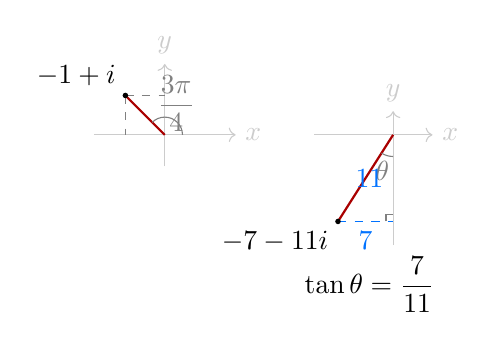
\begin{tikzpicture}[scale=0.5, baseline=(current bounding box.north)]
			% 左：-1+i
			\begin{scope}[shift={(-3.6,0)}]
				\draw[->, gray!40] (-1.8,0) -- (1.8,0) node[right] {$x$};
				\draw[->, gray!40] (0,-0.8) -- (0,1.8) node[above] {$y$};
				\draw[thick, DarkRed] (0,0) -- (-1,1);
				\draw[dashed, gray] (-1,1) -- (-1,0);
				\draw[dashed, gray] (-1,1) -- (0,1);
				\draw[gray] (0.45,0) arc (0:135:0.45);
				\node[gray] at (70:0.85) {$\dfrac{3\pi}{4}$};
				\fill (-1,1) circle (2pt) node[above left] {$-1+i$};
			\end{scope}
			% 右：-7-11i
			\begin{scope}[shift={(2.2,0)}]
				\draw[->, gray!40] (-2,0) -- (1,0) node[right] {$x$};
				\draw[->, gray!40] (0,-2.8) -- (0,0.6) node[above] {$y$};
				\coordinate (P) at (-1.4,-2.2);
				\coordinate (Q) at (0,-2.2);
				\draw[thick, DarkRed] (0,0) -- (P);
				\draw[dashed, SkyBlue] (P) -- (Q);
				\draw[gray] (-0.18,-2.2) -- (-0.18,-2.02) -- (0,-2.02);
				\draw[gray] (237.5:0.55) arc (237.5:270:0.55);
				\node[gray] at (253:0.95) {$\theta$};
				\node[left, SkyBlue] at (0,-1.1) {$11$};
				\node[below, SkyBlue] at (-0.7,-2.2) {$7$};
				\fill (P) circle (2pt) node[below left] {$-7-11i$};
				\node[below] at (-0.6,-2.85) {$\tan\theta=\dfrac{7}{11}$};
			\end{scope}
		\end{tikzpicture}
		
	\end{minipage}
	\begin{knowledge}{三角表示}
		
		任一非零复数都可写成
		\[
		z=|z|(\cos\theta+i\sin\theta),
		\]
		其中$\theta\in\operatorname{Arg}z$为辐角. 三角表示把复数的两个几何量"模"与"辐角"分离出来，是研究乘法、乘方与开方的基础.
		
	\end{knowledge}
	\subsection{复数乘法的几何解释}
	\begin{knowledge}{模相乘、辐角相加}
		
		设$z_1=|z_1|(\cos\theta_1+i\sin\theta_1)$，$z_2=|z_2|(\cos\theta_2+i\sin\theta_2)$，则
		\[
		z_1z_2=|z_1||z_2|\big(\cos(\theta_1+\theta_2)+i\sin(\theta_1+\theta_2)\big).
		\]
		即：积的模等于模之积，积的辐角等于辐角之和.
		
	\end{knowledge}
	\begin{minipage}[t]{0.7\textwidth}
		
		\begin{knowledge}{几何解释}
			
			乘$z_1$的运算：把$z_2$对应的向量逆时针旋转$\arg z_1$，再伸长$|z_1|$倍（如图）.
			
			特别地，乘$i$：$iz$由$z$逆时针旋转$\dfrac{\pi}{2}$得到.
			
		\end{knowledge}
		
	\end{minipage}
	\hfill
	\begin{minipage}[t]{0.3\textwidth}
		
		\centering
		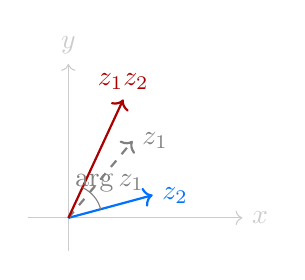
\begin{tikzpicture}[scale=0.85, baseline=(current bounding box.north)]
			\draw[->, gray!40] (-0.6,0) -- (2.6,0) node[right] {$x$};
			\draw[->, gray!40] (0,-0.5) -- (0,2.3) node[above] {$y$};
			\coordinate (Z2) at (1.26,0.34);
			\coordinate (Z1) at (0.96,1.15);
			\coordinate (W) at (0.82,1.77);
			\draw[thick, SkyBlue, ->] (0,0) -- (Z2);
			\draw[thick, gray, dashed, ->] (0,0) -- (Z1);
			\draw[thick, DarkRed, ->] (0,0) -- (W);
			\draw[gray] (15:0.5) arc (15:65:0.5);
			\node[gray] at (40:0.8) {$\arg z_1$};
			\node[SkyBlue, right] at (Z2) {$z_2$};
			\node[gray, right] at (Z1) {$z_1$};
			\node[DarkRed, above] at (W) {$z_1z_2$};
		\end{tikzpicture}
		
	\end{minipage}
	\subsection{复数列}
	\begin{knowledge}{收敛的定义}
		
		设$z_n\in C$（$n\in N$），$\alpha\in C$. 若$\forall\varepsilon>0$，$\exists N\in N$，当$n>N$时恒有$|z_n-\alpha|<\varepsilon$，
		则称数列$\{z_n\}$收敛于$\alpha$，记$\lim\limits_{n\to\infty}z_n=\alpha$.
		
		几何意义：无论邻域$D(\alpha,\varepsilon)$多小，落在其外的$z_n$至多只有有限个.
		
	\end{knowledge}
	\begin{knowledge}{化为实数列}
		
		设$z_n=x_n+iy_n$，$\alpha=a+ib$，则
		\[
		\lim_{n\to\infty}z_n=\alpha \iff \lim_{n\to\infty}x_n=a \text{ 且 } \lim_{n\to\infty}y_n=b.
		\]
		即：复数列收敛等价于实部、虚部两个实数列同时收敛.
		
	\end{knowledge}
	\begin{knowledge}{Cauchy列与完备性}
		
		Def：若$\forall\varepsilon>0$，$\exists N\in N$，当$n,m>N$时恒有$|z_n-z_m|<\varepsilon$，则称$\{z_n\}$为Cauchy列.
		
		Thm：设$z_n=x_n+iy_n$，则$\{z_n\}$是Cauchy列$\iff$ $\{x_n\},\{y_n\}$均为Cauchy列.
		
		Thm（Cauchy收敛准则）：若$\{z_n\}$是Cauchy列，则$\{z_n\}$收敛. 即复数域$C$是完备的.
		
	\end{knowledge}
	\subsection{复级数}
	\begin{knowledge}{级数收敛的定义}
		
		设$\alpha_n\in C$，称$\sum\limits_{n=0}^{\infty}\alpha_n=\alpha_0+\alpha_1+\cdots+\alpha_n+\cdots$为复级数，其部分和为$S_n=\sum\limits_{k=0}^{n}\alpha_k$.
		
		若$\lim\limits_{n\to\infty}S_n=S$，则称该级数收敛于$S$，记$\sum\limits_{n=0}^{\infty}\alpha_n=S$.
		
	\end{knowledge}
	\begin{knowledge}{两个基本定理}
		
		Thm 1：设$\alpha_n=a_n+ib_n$，$S=a+ib$，则
		\[
		\sum_{n=0}^{\infty}\alpha_n=S \iff \sum_{n=0}^{\infty}a_n=a \text{ 且 } \sum_{n=0}^{\infty}b_n=b.
		\]
		
		Thm 2（Cauchy准则）：级数$\sum\alpha_n$收敛$\iff$ $\forall\varepsilon>0$，$\exists N(\varepsilon)$，当$n>N$、$p\in N_+$时恒有
		\[
		|\alpha_{n+1}+\alpha_{n+2}+\cdots+\alpha_{n+p}|<\varepsilon.
		\]
		
		注：由Cauchy准则立得级数收敛的必要条件$\alpha_n\to0$（$n\to\infty$）.
		
	\end{knowledge}
	\subsection{复指数函数、Euler公式与De Moivre定理}
	\begin{knowledge}{级数定义}
		
		\[
		e^z=\sum_{n=0}^{\infty}\dfrac{z^n}{n!},\quad
		\sin z=\sum_{n=0}^{\infty}\dfrac{(-1)^n z^{2n+1}}{(2n+1)!},\quad
		\cos z=\sum_{n=0}^{\infty}\dfrac{(-1)^n z^{2n}}{(2n)!}.
		\]
		上述三个级数对一切$z\in C$都收敛.
		
	\end{knowledge}
	\begin{knowledge}{Euler定理与De Moivre定理}
		
		Euler Thm：$e^{iz}=\cos z+i\sin z$；特别地，对实数$\theta$有$e^{i\theta}=\cos\theta+i\sin\theta$.
		于是三角表示可写成指数形式$z=|z|e^{i\theta}$.
		
		De Moivre Thm：$(\cos\theta+i\sin\theta)^m=\cos m\theta+i\sin m\theta$（$m\in Z$）.
		
	\end{knowledge}
	\category{复数开方}
	\begin{question}
		
		求$-8$的全部立方根，即计算$(-8)^{\frac{1}{3}}$.
		
	\end{question}
	\begin{minipage}[t]{0.7\textwidth}
		
		化指数形式：$-8=8(\cos\pi+i\sin\pi)=8e^{i\pi}$.
		\[
		(-8)^{\frac{1}{3}}=\left(8e^{i\pi}\right)^{\frac{1}{3}}=2\,e^{i\frac{\pi+2k\pi}{3}},\quad k=0,1,2.
		\]
		辐角依次取$\dfrac{\pi}{3},\ \dfrac{3\pi}{3}=\pi,\ \dfrac{5\pi}{3}$（若再取$k=3$，得$\dfrac{7\pi}{3}=\dfrac{\pi}{3}+2\pi$，与$k=0$重复）.
		即三个根为
		\[
		w_0=1+\sqrt{3}\,i,\quad w_1=-2,\quad w_2=1-\sqrt{3}\,i.
		\]
		几何上它们落在以原点为心、半径$2$的圆上，相邻两根辐角相差$\dfrac{2\pi}{3}$，恰构成正三角形.
		
	\end{minipage}
	\hfill
	\begin{minipage}[t]{0.3\textwidth}
		
		\centering
		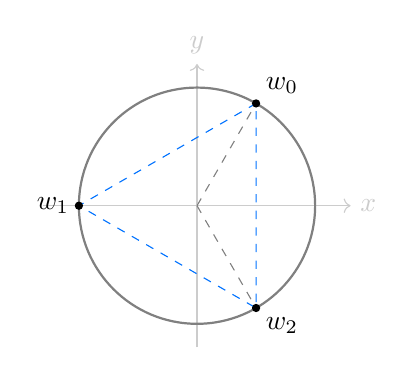
\begin{tikzpicture}[scale=0.75, baseline=(current bounding box.north)]
			\draw[->, gray!40] (-2.6,0) -- (2.6,0) node[right] {$x$};
			\draw[->, gray!40] (0,-2.4) -- (0,2.4) node[above] {$y$};
			\draw[thick, gray] (0,0) circle (2);
			\coordinate (W0) at (1,1.732);
			\coordinate (W1) at (-2,0);
			\coordinate (W2) at (1,-1.732);
			\draw[dashed, SkyBlue] (W0) -- (W1) -- (W2) -- cycle;
			\draw[dashed, gray] (0,0) -- (W0);
			\draw[dashed, gray] (0,0) -- (W2);
			\fill (W0) circle (2pt) node[above right] {$w_0$};
			\fill (W1) circle (2pt) node[left] {$w_1$};
			\fill (W2) circle (2pt) node[below right] {$w_2$};
		\end{tikzpicture}
		
	\end{minipage}
	\section{第二讲\quad 复平面的拓扑与紧性}
	\subsection{邻域、内点、直径与距离}
	\begin{knowledge}{邻域与去心邻域}
		
		邻域：$D(a,r)=\{z:\ |z-a|<r\}$，即以$a$为心、$r$为半径的开圆盘.
		
		去心邻域：$D^{\circ}(a,r)=D(a,r)\setminus\{a\}=\{z:\ 0<|z-a|<r\}$.
		
	\end{knowledge}
	\begin{minipage}[t]{0.7\textwidth}
		
		\begin{knowledge}{内点与开集}
			
			设$E\subset C$，$a\in C$. 若$\exists r>0$，使$D(a,r)\subset E$，则称$a$为$E$的内点.
			
			若$E$的每一点都是内点，则称$E$为开集.
			
		\end{knowledge}
		
	\end{minipage}
	\hfill
	\begin{minipage}[t]{0.3\textwidth}
		
		\centering
		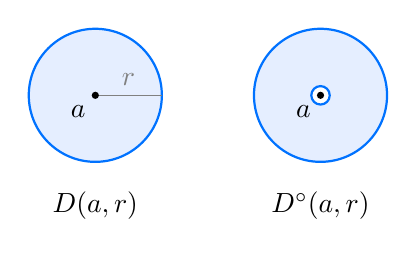
\begin{tikzpicture}[scale=0.65, baseline=(current bounding box.north)]
			\begin{scope}[shift={(-2.2,0)}]
				\fill[LightBlue] (0,0) circle (1.3);
				\draw[thick, SkyBlue] (0,0) circle (1.3);
				\draw[gray] (0,0) -- (1.3,0) node[midway, above] {$r$};
				\fill (0,0) circle (2pt) node[below left] {$a$};
				\node[below] at (0,-1.7) {$D(a,r)$};
			\end{scope}
			\begin{scope}[shift={(2.2,0)}]
				\fill[LightBlue] (0,0) circle (1.3);
				\fill[white] (0,0) circle (0.18);
				\draw[thick, SkyBlue] (0,0) circle (1.3);
				\draw[thick, SkyBlue] (0,0) circle (0.18);
				\fill (0,0) circle (2pt) node[below left] {$a$};
				\node[below] at (0,-1.7) {$D^{\circ}(a,r)$};
			\end{scope}
		\end{tikzpicture}
		
	\end{minipage}
	\begin{knowledge}{直径与距离}
		
		直径：$\operatorname{diam}E=\sup\{|z_1-z_2|:\ z_1,z_2\in E\}$.
		
		距离：$d(E,F)=\inf\{|z_1-z_2|:\ z_1\in E,\ z_2\in F\}$.
		
		补充：$E$有界$\iff$ $\operatorname{diam}E<+\infty$.
		
	\end{knowledge}
	\subsection{Cantor定理}
	\begin{minipage}[t]{0.7\textwidth}
		
		\begin{knowledge}{Cantor Thm}
			
			设$F_n\subset C$（$n=0,1,2,\cdots$）为一列闭集，满足
			\[
			F_0\supset F_1\supset F_2\supset\cdots,\quad \lim_{n\to\infty}\operatorname{diam}F_n=0.
			\]
			则$\bigcap\limits_{n=0}^{\infty}F_n$是单点集，即存在唯一的$z_0$属于一切$F_n$.
			
		\end{knowledge}
		
	\end{minipage}
	\hfill
	\begin{minipage}[t]{0.3\textwidth}
		
		\centering
		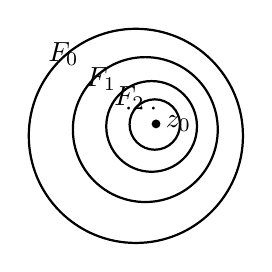
\begin{tikzpicture}[scale=0.8, baseline=(current bounding box.north)]
			\draw[thick] (0,0) circle (1.7);
			\draw[thick] (0.15,0.1) circle (1.15);
			\draw[thick] (0.25,0.15) circle (0.72);
			\draw[thick] (0.3,0.18) circle (0.4);
			\fill (0.32,0.19) circle (2pt) node[right] {$z_0$};
			\node at (-1.15,1.3) {$F_0$};
			\node at (-0.55,0.9) {$F_1$};
			\node at (-0.1,0.6) {$F_2$};
			\node at (0.12,0.42) {$\cdots$};
		\end{tikzpicture}
		
	\end{minipage}
	\subsection{紧性}
	\begin{knowledge}{开覆盖与紧集}
		
		Def 开覆盖：设$E\subset C$，$\mathscr{F}$为开集族. 若$E$的每一点至少属于$\mathscr{F}$中某个开集，则称$\mathscr{F}$为$E$的一个开覆盖.
		
		有限覆盖性质：从$E$的任一开覆盖中，总可选出有限个开集$G_1,\cdots,G_n$，使$E\subset\bigcup\limits_{k=1}^{n}G_k$.
		
		Def 紧集：具有有限覆盖性质的集$E$称为紧集.
		
	\end{knowledge}
	\begin{knowledge}{Heine-Borel Thm}
		
		设$E\subset C$，则$E$有界且闭$\iff$ $E$紧.
		
		（该定理表明在复平面上"有界闭集"与"紧集"等价，是判断紧性的核心准则.）
		
	\end{knowledge}
	\begin{knowledge}{Bolzano-Weierstrass Thm}
		
		凡有界无穷集至少有一个极限点（聚点）；
		
		任意有界序列至少有一个收敛的子序列.
		
	\end{knowledge}
	\begin{minipage}[t]{0.7\textwidth}
		
		\begin{knowledge}{Thm 1.2.5}
			
			设$E$紧、$F$闭，且$E\cap F=\varnothing$，则$\exists a\in E$，$b\in F$，使
			\[
			d(E,F)=|a-b|>0.
			\]
			即：不相交的紧集与闭集之间的距离可由某一对点达到，且必为正数.
			
		\end{knowledge}
		
	\end{minipage}
	\hfill
	\begin{minipage}[t]{0.3\textwidth}
		
		\centering
		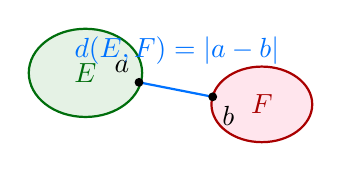
\begin{tikzpicture}[scale=0.8, baseline=(current bounding box.north)]
			\fill[LightGreen] (-1.3,0.2) circle (0.9 and 0.7);
			\draw[thick, DarkGreen] (-1.3,0.2) circle (0.9 and 0.7);
			\fill[LightPink] (1.5,-0.3) circle (0.8 and 0.6);
			\draw[thick, DarkRed] (1.5,-0.3) circle (0.8 and 0.6);
			\coordinate (A) at (-0.45,0.05);
			\coordinate (B) at (0.72,-0.18);
			\draw[thick, SkyBlue] (A) -- (B);
			\fill (A) circle (2pt) node[above left] {$a$};
			\fill (B) circle (2pt) node[below right] {$b$};
			\node[SkyBlue] at (0.15,0.55) {$d(E,F)=|a-b|$};
			\node[DarkGreen] at (-1.3,0.2) {$E$};
			\node[DarkRed] at (1.5,-0.3) {$F$};
		\end{tikzpicture}
		
	\end{minipage}
	\subsection{复球面与扩充复平面}
	\subsubsection{直线与圆周的复方程}
	\begin{minipage}[t]{0.7\textwidth}
		
		\begin{knowledge}{直线的复方程}
			
			过两点$z_1,z_2$的直线$L$的参数式为
			\[
			z=z_1+t(z_2-z_1)\quad(t\in R).
			\]
			由于乘$i$相当于逆时针旋转$90^\circ$，故$i(z_2-z_1)\perp(z_2-z_1)$，
			\[
			z\in L \iff \operatorname{Re}\left[i(z_2-z_1)\cdot\overline{(z-z_1)}\right]=0.
			\]
			利用$\operatorname{Re}w=\dfrac{w+\bar w}{2}$，上式可写成共轭对称形式
			\[
			\left[i(z_2-z_1)\cdot\overline{z-z_1}\right]+\overline{\left[i(z_2-z_1)\cdot\overline{z-z_1}\right]}=0.
			\]
			展开整理即得直线的一般复方程$\bar B z+B\bar z+C=0$（$B\in C$，$B\neq0$，$C\in R$）.
			
		\end{knowledge}
		
	\end{minipage}
	\hfill
	\begin{minipage}[t]{0.3\textwidth}
		
		\centering
		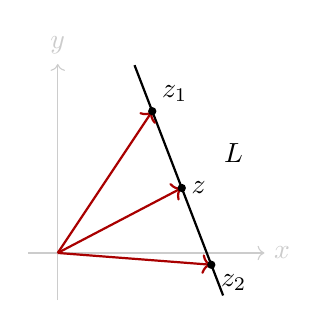
\begin{tikzpicture}[scale=0.75, baseline=(current bounding box.north)]
			\draw[->, gray!40] (-0.5,0) -- (3.5,0) node[right] {$x$};
			\draw[->, gray!40] (0,-0.8) -- (0,3.2) node[above] {$y$};
			\coordinate (Z1) at (1.6,2.4);
			\coordinate (Z2) at (2.6,-0.2);
			\coordinate (Z) at (2.1,1.1);
			\draw[thick] (1.3,3.18) -- (2.8,-0.72);
			\draw[thick, DarkRed, ->] (0,0) -- (Z1);
			\draw[thick, DarkRed, ->] (0,0) -- (Z);
			\draw[thick, DarkRed, ->] (0,0) -- (Z2);
			\fill (Z1) circle (2pt) node[above right] {$z_1$};
			\fill (Z) circle (2pt) node[right] {$z$};
			\fill (Z2) circle (2pt) node[below right] {$z_2$};
			\node[right] at (2.65,1.7) {$L$};
		\end{tikzpicture}
		
	\end{minipage}
	\begin{minipage}[t]{0.7\textwidth}
		
		\begin{knowledge}{圆周的复方程}
			
			圆周$\partial D(z_0,R)$，圆心$z_0=a+ib$，其参数方程为
			\[
			z-(a+ib)=Re^{i\theta}\quad(0\le\theta\le2\pi).
			\]
			由$|z-z_0|^2=R^2$，即$(z-z_0)\overline{(z-z_0)}=R^2$，展开得
			\[
			z\bar z-\bar z_0 z-z_0\bar z+|z_0|^2-R^2=0.
			\]
			故圆周可表为统一形式
			\[
			Az\bar z+\bar B z+B\bar z+C=0\quad(A,C\in R,\ B\in C,\ A\neq0),
			\]
			其中以$-\dfrac{B}{A}$为圆心，$R=\dfrac{\sqrt{|B|^2-AC}}{|A|}$为半径（需$|B|^2-AC>0$）.
			反之，当$A=0$、$B\neq0$时该形式表示直线：直线与圆周共用同一复方程.
			
		\end{knowledge}
		
	\end{minipage}
	\hfill
	\begin{minipage}[t]{0.3\textwidth}
		
		\centering
		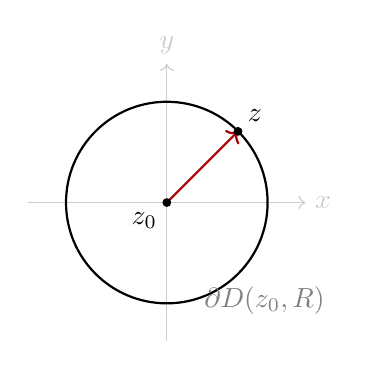
\begin{tikzpicture}[scale=0.8, baseline=(current bounding box.north)]
			\draw[->, gray!40] (-2.2,0) -- (2.2,0) node[right] {$x$};
			\draw[->, gray!40] (0,-2.2) -- (0,2.2) node[above] {$y$};
			\draw[thick] (0,0) circle (1.6);
			\coordinate (Z0) at (0,0);
			\coordinate (Z) at (1.13,1.13);
			\draw[thick, DarkRed, ->] (Z0) -- (Z);
			\fill (Z0) circle (2pt) node[below left] {$z_0$};
			\fill (Z) circle (2pt) node[above right] {$z$};
			\node[gray] at (1.55,-1.55) {$\partial D(z_0,R)$};
		\end{tikzpicture}
		
	\end{minipage}
	\subsubsection{Riemann球面与球极投影}
	\begin{minipage}[t]{0.7\textwidth}
		
		\begin{knowledge}{Riemann球面}
			
			取单位球面$S=\{(x,y,u)\in R^3:\ x^2+y^2+u^2=1\}$，北极$N(0,0,1)$；把复平面取为赤道面$u=0$，即$z=x+iy\leftrightarrow(x,y,0)$.
			
			对$z(x,y,0)$，连$Nz$交球面于另一点$P(x',y',u')$，于是$C$与$S\setminus\{N\}$之间建立一个双射；再定义无穷远点$z=\infty$，记$C_\infty=C\cup\{\infty\}$，并规定$\infty\leftrightarrow N$，即得双射$f:C_\infty\to S$（球极投影）.
			
			投影公式：
			\[
			x'=\dfrac{z+\bar z}{|z|^2+1},\quad
			y'=\dfrac{z-\bar z}{i(|z|^2+1)},\quad
			u'=\dfrac{|z|^2-1}{|z|^2+1};
			\]
			即
			\[
			x'+iy'=\dfrac{2z}{1+|z|^2},\quad 1-u'=\dfrac{2}{1+|z|^2};
			\]
			逆变换为
			\[
			z=\dfrac{x'+iy'}{1-u'}.
			\]
			（推导用到$x^2+y^2=|z|^2=z\bar z$，$2x=z+\bar z$，$2y=\dfrac{z-\bar z}{i}$.)
			
		\end{knowledge}
		
	\end{minipage}
	\hfill
	\begin{minipage}[t]{0.3\textwidth}
		
		\centering
		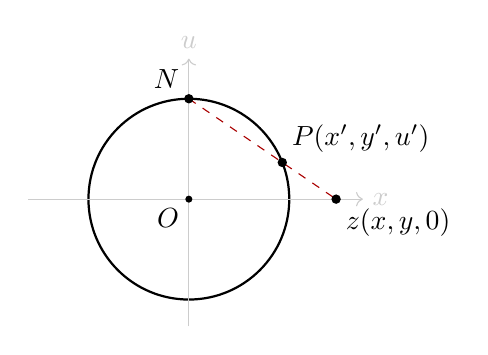
\begin{tikzpicture}[scale=0.85, baseline=(current bounding box.north)]
			\draw[thick] (0,0) circle (1.5);
			\draw[->, gray!40] (-2.4,0) -- (2.6,0) node[right] {$x$};
			\draw[->, gray!40] (0,-1.9) -- (0,2.1) node[above] {$u$};
			\coordinate (N) at (0,1.5);
			\coordinate (Z) at (2.2,0);
			\coordinate (P) at (1.396,0.548);
			\draw[dashed, DarkRed] (N) -- (Z);
			\fill (N) circle (2pt) node[above left] {$N$};
			\fill (P) circle (2pt) node[above right] {$P(x',y',u')$};
			\fill (Z) circle (2pt) node[below right] {$z(x,y,0)$};
			\fill (0,0) circle (1.5pt) node[below left] {$O$};
		\end{tikzpicture}
		
	\end{minipage}
	\begin{knowledge}{球面圆周方程}
		
		球面上的圆周是$S$与平面的交线：
		\[
		\begin{cases}
			x'^2+y'^2+u'^2=1,\\
			a_1x'+a_2y'+a_3u'=a,
		\end{cases}
		\quad a_1^2+a_2^2+a_3^2=1,\ |a|<1.
		\]
		将投影公式代入平面方程，整理得
		\[
		Az\bar z+\bar B z+B\bar z+C=0,
		\]
		其中$A=a_3-a$，$B=a_1+ia_2$，$C=-(a_3+a)$（$A,C$为实，$B$为复）.
		
		1$^\circ$ 当$|B|^2-AC>0$且$A\neq0$时：为$C$上一个圆周；
		
		2$^\circ$ 若$S$上圆周过北极，则$a_3=a$，$A=0$，球极投影为$C$上一直线（半径为$\infty$的"圆周"）：
		\[
		(a_1+ia_2)\bar z+\overline{(a_1+ia_2)}z-2a=0;
		\]
		
		3$^\circ$ $a=0$（最大圆周，即大圆）$\iff A+C=-2a=0$.
		
		结论：球极投影下，球面上的圆周与扩充复平面上的圆周或直线一一对应.
		
	\end{knowledge}
	\subsubsection{球面距离}
	\begin{minipage}[t]{0.7\textwidth}
		
		\begin{knowledge}{球面距离（弦距）}
			
			设$z_1,z_2\in C_\infty$分别对应$P_1(x_1',y_1',u_1')$，$P_2(x_2',y_2',u_2')\in S$，定义球面距离
			\[
			d_S(z_1,z_2)=\sqrt{(x_1'-x_2')^2+(y_1'-y_2')^2+(u_1'-u_2')^2}.
			\]
			代入投影公式化简得
			\[
			d_S(z_1,z_2)=\dfrac{2|z_1-z_2|}{\sqrt{(|z_1|^2+1)(|z_2|^2+1)}};
			\]
			特别地，
			\[
			d_S(z,\infty)=\sqrt{x'^2+y'^2+(u'-1)^2}=\dfrac{2}{\sqrt{|z|^2+1}}.
			\]
			注：$d_S(z_n,\infty)\to0 \iff |z_n|\to\infty$，即$z_n\to\infty$可用球面距离刻画；$d_S$使$C_\infty$成为紧度量空间.
			
		\end{knowledge}
		
	\end{minipage}
	\hfill
	\begin{minipage}[t]{0.3\textwidth}
		
		\centering
		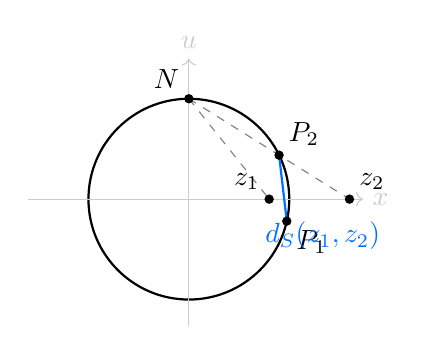
\begin{tikzpicture}[scale=0.85, baseline=(current bounding box.north)]
			\draw[thick] (0,0) circle (1.5);
			\draw[->, gray!40] (-2.4,0) -- (2.6,0) node[right] {$x$};
			\draw[->, gray!40] (0,-1.9) -- (0,2.1) node[above] {$u$};
			\coordinate (N) at (0,1.5);
			\coordinate (Z1) at (1.2,0);
			\coordinate (Z2) at (2.4,0);
			\coordinate (P1) at (1.463,-0.329);
			\coordinate (P2) at (1.348,0.657);
			\draw[dashed, gray] (N) -- (Z1);
			\draw[dashed, gray] (N) -- (Z2);
			\draw[thick, SkyBlue] (P1) -- (P2);
			\fill (N) circle (2pt) node[above left] {$N$};
			\fill (P1) circle (2pt) node[below right] {$P_1$};
			\fill (P2) circle (2pt) node[above right] {$P_2$};
			\fill (Z1) circle (2pt) node[above left] {$z_1$};
			\fill (Z2) circle (2pt) node[above right] {$z_2$};
			\node[SkyBlue] at (2.0,-0.55) {$d_S(z_1,z_2)$};
		\end{tikzpicture}
		
	\end{minipage}
	
	
	
	
\end{document}